%
% 2-tangentialvektoren.tex -- Tangentialvektoren
%
% (c) 2024 Prof Dr Andreas Müller
%
\section{Tangentialvektoren
\label{buch:koordinaten:section:tangentialvektoren}}
\kopfrechts{Tangentialvektoren}
Das elektrische Feld übt auf eine Testladung eine Kraft aus, die
proportional zur Ladung ist.
Diese Kräfte stellt man sich gerne als ein Vektorfeld vor, doch
in welchem Raum sind diese Vektoren zu finden?
Die Kraft verursacht eine Beschleunigung und verändert damit 
die Geschwindigkeit.
%
% fig-tangentialvektoren.tex
%
% (c) 2025 Prof Dr Andreas Müller
%
\begin{figure}
\centering
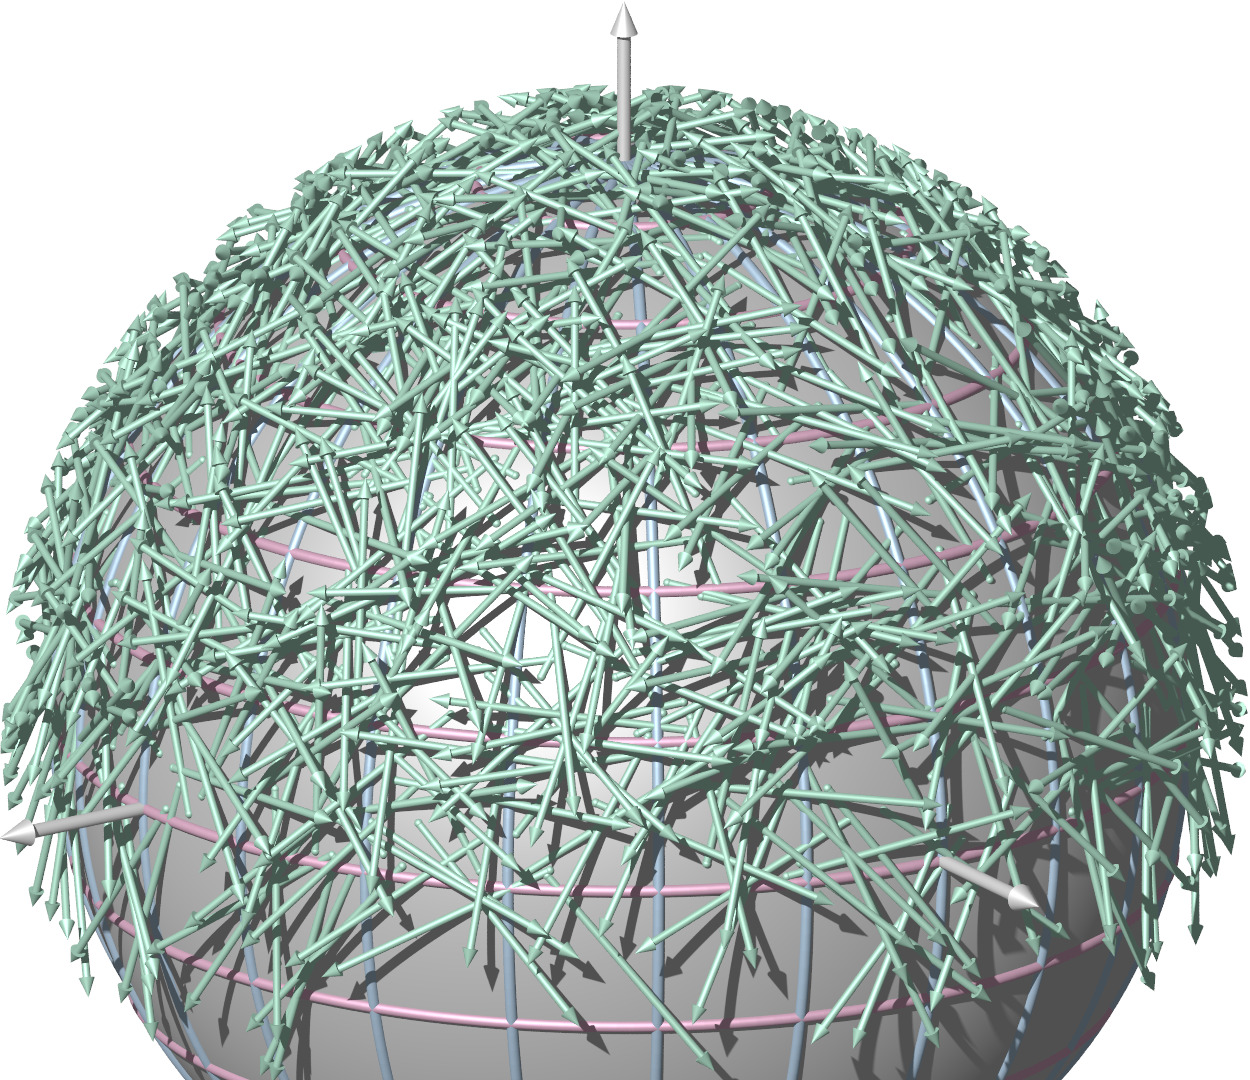
\includegraphics[width=10cm]{chapters/020-koordinaten/images/tangentialvektoren.jpg}
\caption{Darstellung von tausend Tangentialvektoren an die Nordhalbkugel.
Ganz offensichtlich sind die Tangentialvektoren nicht Teil der Kugel.
\label{buch:koordinaten:fig:tangentialvektoren}}
\end{figure}
%
Als erstes muss daher der Geschwindigkeitsvektor konstruiert werden,
der tangential an die Bahnkurve der Testladung verläuft.
An dieser naheliegenden und üblichen Darstellung ist aber eigentlich
falsch, dass der Geschwindigkeitsvektor gar nicht im gleichen Raum
dargestellt werden kann
(Abbildung~\ref{buch:koordinaten:fig:tangentialvektoren}).
Die Masseinheit der Komponenten des Geschwindigkeitsvektors ist
[Länge/Zeit], während die Koordinaten die Masseinheit [Länge] haben.
Solange man das Koordinatensystem und damit die Masseinheiten nicht
wechselt, mag die Konfusion in Grenzen bleiben.
Da aber alle Gesetzmässigkeiten auf eine koordinatensystemunabhängige
Art formuliert werden müssen, bedarf auch das Konzept des Tangentialvektors
einer Reevaluation.

%
% Kurven
%
\subsection{Kurven}
Für ein kartesisches Koordinatensystem in der Ebene ist klar, welche
Richtung man den Koordinatenachsen zuordnen kann.
Es ist üblich, die Koordinatenachsen als Vektoren in der Ebene
zu zeichnen.
Die Idee einer geraden Koordinatenachse ist nicht mehr anwendbar,
wenn beliebige Koordinatensysteme verwendet werden sollen.
Bei der Umrechnung zwischen Koordinatensystemen entstehen unweigerlich
gekrümmte Koordinatenlinien.
Es braucht also etwas mehr Sorgfalt, die Idee der {\em Richtung}
Koordinatenunabhängig zu definieren.

\subsubsection{Differenzierbare Kurven}
Im Folgenden gehen wir on einer Menge $Y$ mit einer $n$-dimensionalen
differenzierbaren Struktur aus.
Statt uns auf die in der Einleitung angedeuteten gekrümmten
Koordinatenlinien zu beschränken, möchten wir beliebige Kurven
definieren.
Kurven sehen in der Umgebung eines Punktes wie die reelle Achse
$\mathbb{R}$ aus.
Tatsächlich können wir jedes Intervall $X=(a,b)\subset\mathbb{R}$ als
eine Menge mit einer differenzierbaren Struktur betrachten, indem
wir die Einbettung
\[
\varphi
\colon
X=(a,b) \hookrightarrow \mathbb{R}
:
x\mapsto x
\]
als Koordinatensystem verwenden (Der ``Haken'' am Abbildungspfeil
soll die Einbettung symbolisieren).
Die Koordinatenwechselabbildung zu einem alternativen Koordinatensystem
auf dem Intervall ist eine streng monoton wachsende, differenzierbare
Funktion, deren Ableitung nirgends verschwindet.
In einem Punkt $x_0\in (a,b)$ sind Koordinatenwechsel daher sehr
einfach: Sie sind nur von 0 verschiedene Zahlen.
Diese Einfachheit erlaubt uns, zur Vereinfachung der Notation die Menge
$(a,b)$ mit den Koordinatenwerten zu identifizieren.

\begin{definition}[differenzierbare Kurve]
Eine {\em differenzierbare Kurve}
\index{differenzierbare Kurve}%
\index{Kurve, differenzierbar}%
ist eine differenzierbare Abbildung
\[
\gamma
\colon
X = (a,b) \to Y
:
t \mapsto \gamma(t).
\]
\end{definition}

Durch Zusammensetzen der Abbildung $\gamma$ mit einem Koordinatenssystem
$\varphi\colon X\to \mathbb{R}^n$ entsteht eine Abbildung 
\[
\varphi\circ\gamma
\colon
X=(a,b) \to \mathbb{R}^n
:
t \mapsto (\varphi^1\circ \gamma(t),\dots,\varphi^n\circ\gamma(t)),
\]
wobei jede Koordinate $\varphi^i\circ\gamma(t) = \varphi^i(\gamma(t))$
eine differenzierbare Funktion von $t$ ist.

\begin{beispiel}
Die Menge $Y=\mathbb{R}^2$ hat eine differenzierbare Struktur gegeben durch
das kartesische Koordinatensystem
\[
\varphi
\colon
Y\to\mathbb{R}^2
:
(x,y)\mapsto (x,y).
\]
Die Kurve 
\[
\gamma
\colon
\mathbb{R}\to Y
:
t\mapsto (\cos t, \sin t)
\]
ist der Einheitskreis in der Ebene.

Koordinatenwechsel auf dem Urbildbereich $(-\infty,\infty)$ sind durch
Funktionen $f\colon\mathbb{R}\to\mathbb{R}$ gegeben, deren Ableitung
nirgends verschwindet.
Nach dem Koordinatenwechsel ist die Kurven durch die Parametrisierung
\[
t \mapsto (\cos f(t),\sin f(t))
\]
gegeben.

Statt der kartesischen Koordinaten kann man mindestens auf der Teilmenge
$Y=X\setminus (0,0)$ Polarkoordinaten mit der Koordinatenabbildung $\psi$
verwenden.
Die Koordinatenumrechnung von Polarkoordinaten in kartesische Koordinaten
ist
\[
(\varphi, r) \mapsto (r\cos\varphi,r\sin\varphi)
\]
mit der Umkehrung
\[
(x,y) \mapsto \Bigl(\arctan\frac{y}{x},\sqrt{x^2+y^2}\Bigr),
\]
wobei die $\arctan$-Funktion etwas erweitert werden muss, wie es die
in den meisten Programmierbibliotheken durch die Funktion \texttt{atan2}
gemacht wird.

In Polarkoordinaten bekommt die Kurve $\gamma$ die Form
\[
t\mapsto \psi\circ\gamma(t)
=
(t, 1).
\]
Die zweite Koordinaten ist konstant und damit ganz offensichtlich 
differenzierbar.
Die erste Koordinate hat die Ableitung $1$.
\end{beispiel}

Eine Kurve in $Y$ ist also eine Abbildung $X\to Y$.
Sowohl in $X$ wie auch in $Y$ können beliebige Koordinatensysteme
gewählt werden.
Es ist nur sinnvoll über Objekte zu sprechen, welche in dem
Sinne unabhängig sind von der Wahl des Koordinatensystems, dass
auch Umrechnungsformeln zwischen den Koordinatensystemen bereitgestellt
sind.

% XXX Ableitung der Koordinaten

% XXX Koordinatenwechsel und Ableitung


\subsubsection{Tangentiale Kurven}
Das Beispiel illustriert, dass der Begriff der ``Richtung'' einer
Koordinatenachse nicht sinnvoll sein kann.
Im Wertebereich der Koordinatensysteme unterscheidet sich das Bild
der Kurve $\gamma$ grundsätzlich.
Im Koordinatensystem ist $\varphi\circ\gamma$ eine gekrümmte Kurve,
während sie im Polarkoordinatensystem in der Umgebung des Punktes
$(1,0)$ die Gerade $r=1$ ist.
Die Kurve durch einen Punkt von $Y$ kann also keine koordinatenunabhängig
Bedeutung haben, aber für die Richtung der Kurve in einem Punkt ist
dies möglich.
Es muss daher definiert werden, wann zwei Kurven die gleiche Richtung
in einem gemeinsamen Punkt haben.


%
% fig-kurve.tex
%
% (c) 2024 Prof Dr Andreas Müller
%
\begin{figure}
\centering
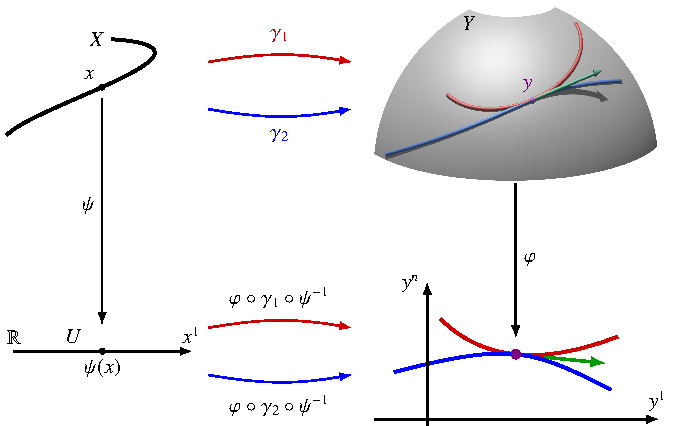
\includegraphics{chapters/020-koordinaten/images/kurve.pdf}
\caption{Die Kurven $\gamma_1$ und $\gamma_2$ sind tangential im
Punkt $y$, wenn $\gamma_1(x)=y=\gamma_2(x)$ und ausserdem die
Ableitungen der Zusammensetzungen $\varphi\circ\gamma_i\circ\psi^{-1}$
in $\psi(x)$ übereinstimmen.
Es ist nicht sinnvoll, von einem Tangentialvektor ``in $Y$'' (grün,
oben rechts) zu sprechen, erst durch das Koordinatensystem kann
das Konzept des Tangentialvektors konsistent definiert werden.
\label{buch:koordinaten:tangentialvektoren:fig:kurve}}
\end{figure}
%

\begin{definition}[tangentiale Kurven]
Zwei Kurven $\gamma_i\colon X\to Y$, $i=1,2$, sind
{\em tangential} im Punkt $y\in Y$, wenn
$\gamma_i(x) = y$, $i=1,2$, und
in jeder Karte
$\varphi\colon Y\to\mathbb{R}^n$ und für die Parametrisierung
$\psi\colon X\to \mathbb{R}$ mit Parameter $x^1\in\mathbb{R}$ 
im Punkt $\psi(x)$ die Ableitungen der Abbildungen
\[
\varphi
\circ
\gamma_i
\circ
\psi^{-1}
\colon
U\to\mathbb{R}^n
\]
übereinstimmen, d.~h.
\begin{equation}
\frac{d}{dx^1}
\bigl(\varphi\circ\gamma_1\circ\psi^{-1}\bigr)(\psi(x))
=
\frac{d}{dx^1}
\bigl(\varphi\circ\gamma_2\circ\psi^{-1}\bigr)(\psi(x))
\label{buch:koordinaten:tangentialvektoren:eqn:tangential}
\end{equation}
für $x^1=\psi(x)$.
\end{definition}

Kurven sind also tangential in einem Punkt, wenn sie sich in jedem
Koordinatensystem mit der gleichen momentanen Geschwindigkeit
durch den Punkt im Koordinateraum bewegen.
Die Abbildung~\ref{buch:koordinaten:tangentialvektoren:fig:kurve}
macht auch deutlich, dass es nicht sinnvoll ist, von einem
Tangentialvektor im Punkt $y$ an die Kurven ``in $Y$'' zu sprechen.
Der grün eingezeichnete Tangentialvektor ist nicht Teil von $Y$.
Er hängt von der Art der für die graphische Darstellung notwendigen
Einbettung von Y in den dreidimensionalen Raum ab.
Eine rein geometrische Definition des Tangentialvektors ist also
nicht möglich.
Erst im Koordinatensystem, also nach der Abbildung mit $\varphi$,
entsteht ein Tangentialvektor, mit dem man in $\mathbb{R}^n$
rechnen kann, doch dieser Tangentialvektor hängt notwendigerweise
vom Koordinatensystem ab.
Es muss daher zusätzlich geklärt werden, wie sich der Tangentialvektor
ändert, wenn man ein anderes Koordinatensystem verwendet.

%
% Tangentialvektoren
%
\subsection{Tangentialvektoren}
Die Eigenschaft von Kurven, im Punkt $y$ tangential zu sein, ist
eine Äquivalenzrelation.
In einem Koordinatensystem haben die tangentiale Kurven gemäss
Abbildung~\ref{buch:koordinaten:tangentialvektoren:fig:kurve}
den grünen Tangentialvektor {\em im Koordinatensystem} gemeinsam.
Die folgende, sehr abstrakte Definition eines Tangentialvektors
von $Y$ ist unabhängig von einer Einbettung von $Y$ in einen
grösseren Raum für Darstellungszwecke.

\begin{definition}[Tangentialvektor]
\label{buch:koordinaten:tangentialvektoren:def:tangentialvektor}
Ein Tangentialvektor $V$ im Punkt $y\in Y$ ist die Menge aller Kurven, die
im Punkt $y$ tangential sind.
In einem Koordinatensystem $\varphi$ ist der Tangentialvektor an die Kurve
$\gamma$ durch die Komponenten
\[
u^i
=
\frac{d}{dx^1} \varphi^i(\gamma(\psi(x^1))) \bigg|_{x^1 = \psi(x)}
\]
gegeben.
Der Tangentialvektor an die Kurve $\gamma$ an der Stelle $x$
wird auch als $T_x\gamma\cdot e_1$ bezeichnet.
\end{definition}

Verwendung eines anderen Koordinatensystems $\varphi'$ anstelle von
$\varphi$ bedeutet, dass die Komponenten des Tangentialvektors
an die Kurve mit der Koordinatentransformation
$g=\varphi'\circ\varphi^{-1}$ umgerechnet werden müssen.
Im neuen Koordinatensystem sind die Komponenten
\begin{align}
u^{\prime i}
&=
\frac{d}{dx^1}
\varphi^{\prime i}(\gamma(\psi^{-1}(x^1))) \bigg|_{x^1=\psi(x)}
\notag
\\
&=
\frac{d}{dx^1}
(\varphi'\circ\varphi^{-1})^i\circ \varphi\circ\gamma\circ\psi^{-1}(x^1)
\bigg|_{x^1=\psi(x)}
\notag
\\
&=
\frac{d}{dx^1} g^i\circ(\varphi\circ\gamma\circ\psi^{-1})(x^1)
\bigg|_{x^1=\psi(x)}
\notag
\\
&=
\sum_{k=1}^n
\frac{\partial g^i}{\partial y^k}(\varphi(y))
\cdot
\frac{d}{dx^1}\varphi^k(\circ(\psi^{-1})) 
\bigg|_{x^1=\psi(x)}
\notag
\\
&=
\sum_{k=1}^n
\frac{\partial g^i}{\partial y^k}(\varphi(y))
\cdot
u^k.
\label{buch:koordinaten:tangentialvektoren:eqn:tangentialtransformation}
\end{align}
Die Ableitungsterme in
\eqref{buch:koordinaten:tangentialvektoren:eqn:tangentialtransformation}
sind die Einträge der Jacobi-Matrix der Abbildung $g$.

Man beachte, dass der Index $i$ auf der linken und der rechten 
Seite des Ausdrucks für $u^{\prime i}$ als oberer Index vorkommt.
Der Summationsindex kommt in den Faktoren $u^k$ als oberer Index
vor, während er in der Jacobi-Matrix unter dem Bruchstrich steht.
Eine Dimensionsüberlegung kann illustrieren, dass der Position unter
dem Bruchstrich eine andere Bedeutung zukommt.
Wird nämlich die Masseinheit für die Koordinaten $y$ durch eine kleinere
Einheit ersetzt, werden die Komponenten $u^k$ des Tangentialvektors
grösser.
Die Ableitungen nach $y^k$ werden aber um den gleichen Faktor kleiner.
Im Ausdruck 
\eqref{buch:koordinaten:tangentialvektoren:eqn:tangentialtransformation}
heben sich diese beiden Faktoren auf und er bleibt unverändert.
Dies ist auch notwendig, denn die Komponenten $u^{\prime i}$ dürfen
sich nicht verändern, wenn man sie ausgehend von einem anderen
Koordinatensystem zu berechnen versucht.

Um anzudeuten, dass sich die Ableitungen nach den $y^k$ anders verhalten
als die Komponenten des Tangentialvektors oder die Koordinaten selbst,
unterscheiden wir sie durch die Position des Index.
Wir schreiben daher im Folgenden die Jacobi-Matrix als
\[
J^i\mathstrut_k
=
\frac{\partial g^i}{\partial y^k}.
\]
Im Ableitungsoperator nach $y^k$ muss also der Index $k$ auch als ein 
unterer Index betrachtet werden.
Wir kürzen die Ableitungsoperatoren daher auch als
\[
\partial_k = \frac{\partial}{\partial y^k}
\]
ab.
Die Jacobi-Matrix lässt sich damit als
\[
J^i\mathstrut_k = \partial_k g^i
\]
schreiben und der Ausdruck
\eqref{buch:koordinaten:tangentialvektoren:eqn:tangentialtransformation}
wird zu
\begin{equation}
u^{\prime i}
=
\sum_{k=1}^n J^i\mathstrut_k \cdot u^k
=
\sum_{k=1}^n \partial_kg^i\cdot u^k.
\label{buch:koordinaten:tangentialvektoren:eqn:transformationkurz}
\end{equation}

Ein einzelner Eintrag des Tangentialvektors oder der Jacobi-Matrix
kann nicht sinnvoll die Basis eines Naturgesetzes sein, weil er bei
einer Koordinatentransformation durch andere Einträge oder Linearkombenationen
von Einträgen ersetzt wird.
Nur die Kombination
\eqref{buch:koordinaten:tangentialvektoren:eqn:transformationkurz},
in der für jeden Index $i$ nur die Summe über alle $k$ erstreckt
wird, ist unabhängig von der Wahl des $y^k$-Koordinatensystems.
Daher ist es keine Einschränkung, diese Summierung automatisch
vorzunehmen, wann immer ein oberer und untere Index in einem Ausdruck
auftreten.

\begin{definition}[einsteinsche Summenkonvention]
Kommt in einem Ausdruck der gleiche Index als oberer und als unterer
Index vor, dann wird über diesen Index summiert.
\end{definition}

Die Matrizenmultiplikation der Matrizen $A$ mit den Einträgen $a_{ik}$ und
$B$ mit den Einträgen $b_{kl}$ liefert die Einträge der Produktmatrix
$C=AB$ mit den Einträgen $c_{il}$ als Summe
\[
c_{il}
=
\sum_{k=1}^n
a_{ik} b_{kl}.
\]
Die einsteinsche Summenkonvention legt nahe, dass Matrizen mit oberen
und unteren Indizes geschrieben werden sollten, so dass man die
Elemente von $C$ als
\[
c^i\mathstrut_l
=
a^i\mathstrut_k\,
b^k\mathstrut_l
\]
berechnen kann, wo implizit über $k$ summiert wird.
Der Zeilenindex wird darin als oberer Index geschrieben, so wie
die Komponenten von Spaltenvektoren, auf denen Matrizen wirken können, 
ebenfalls als obere Indizes geschrieben werden.
Der Zeilenindex bekommt daher den Platz als unterer Index.

Der Ausdruck
\eqref{buch:koordinaten:tangentialvektoren:eqn:transformationkurz}
kann daher kompakter als
\[
u^{\prime i}
=
J^i\mathstrut_k \cdot u^k
=
\partial_kg^i\cdot u^k
\]
geschrieben werden.

%
% Tangentialvektoren als Spaltenvektoren
%
\subsection{Tangentialvektoren als Spaltenvektoren}
In einem Koordinatensystem ist ein Tangentialvektor durch die Komponenten
$u^k$ gegeben.
Bei einem Koordinatenwechsel werden diese Komponenten mit der
Jacobi-Matrix multipliziert.
In Matrix-Notation wird dies als
\[
u^{\prime i}
=
\sum_{k=1}^n
J^i\mathstrut_k \cdot u^k
\qquad\Rightarrow\qquad
\begin{pmatrix}
u^{\prime 1}\\
u^{\prime 2}\\[-2pt]
\vdots\\
u^{\prime n}
\end{pmatrix}
=
\bgroup
\renewcommand{\arraystretch}{1.8}
\begin{pmatrix}
\displaystyle\frac{\partial  g^1}{\partial y^1}&
\displaystyle\frac{\partial  g^1}{\partial y^2}&
\dots&
\displaystyle\frac{\partial  g^1}{\partial y^n}
\\[-2pt]
%\displaystyle\frac{\partial  g^2}{\partial y^1}&
%\displaystyle\frac{\partial  g^2}{\partial y^2}&
%\dots&
%\displaystyle\frac{\partial  g^2}{\partial y^n}
%\\
\vdots&\vdots&\ddots&\vdots\\
\displaystyle\frac{\partial  g^n}{\partial y^1}&
\displaystyle\frac{\partial  g^n}{\partial y^2}&
\dots&
\displaystyle\frac{\partial  g^n}{\partial y^n}
\end{pmatrix}
\egroup
\begin{pmatrix}
u^{1}\\
u^{2}\\
\vdots\\[-2pt]
u^{n}
\end{pmatrix}
\]
geschrieben.
Tangentialvektoren sind daher als Spaltenvektoren zu betrachten.
\index{Spaltenvektoren}%

%
% Koordinatenlinien
%
\subsection{Koordinatenlinien
\label{buch:koordinaten:tangentialvektoren:subsection:koordinatenlinien}}
Sei $(X,\varphi)$ ein Koordinatensystem auf $X$.
Mit der inversen Abbildung $\varphi^{-1}$ lassen sich durch jeden Punkt
$x_0\in X$ Kurven finden, entlang denen sich nur eine Koordinate
ändert.
Sei also $x_0\in X$ ein beliebiger Punkt in $X$.
Die Abbildung
\[
\gamma_k
\colon
(-\varepsilon,\varepsilon)
\to
X
:
t
\mapsto
\gamma_k(t)
=
\varphi^{-1}(x_0^1,\dots,x_0^k+t,x_0^n)
\]
ist eine Kurve in $X$.
Sie heisst die Koordinatenlinie der Koordinaten $x^k$.

Die Zusammensetzung von $\gamma_k$ mit $\varphi$ ergibt für die
einzelnen Koordinaten
\[
\varphi^i\circ\gamma_k(t)
=
\begin{cases}
x_0^i+t&\qquad\text{falls $k=i$} \\
x_0^i  &\qquad\text{sonst}.
\end{cases}
\]
Die Ableitung nach $t$ ergibt die Komponenten des Tangentialvektors im
Punkt $x_0$ als
\[
\frac{d}{dt}\varphi^i\circ\gamma_k(t)
\bigg|_{t=0}
=
\begin{cases}
1&\qquad \text{falls $k=i$}\\
0&\qquad\text{sonst.}
\end{cases}
\qquad\Rightarrow\qquad
T_0\gamma_k \cdot e_1 = e_k.
\]
Die Koordinatenlinie $\gamma_k$ hat in jedem Punkt also den
Standardbasisvektor $e_k$ als Tangentialvektor.
